\documentclass[11pt, a4paper]{article}
\usepackage[letterpaper, portrait, margin=0.5in]{geometry}
\usepackage[english]{babel}  % force American English hyphenation patterns
\usepackage{amsmath,mathtools}

\usepackage{graphicx}
\usepackage{wrapfig}


\begin{document}
\title{Chapter 15 Periodic Motion}
\author{Apostolos Delis}
\date{\today}
\maketitle

\tableofcontents
\section[15.1, Types of Mechanical Wabves]{Types of Mechanical Waves}
\begin{itemize}
    \item A mechanical wave is a disturbance that travels through some material or
        substance called the medium for the wave.
    \item There are three varieties of mechanical waves

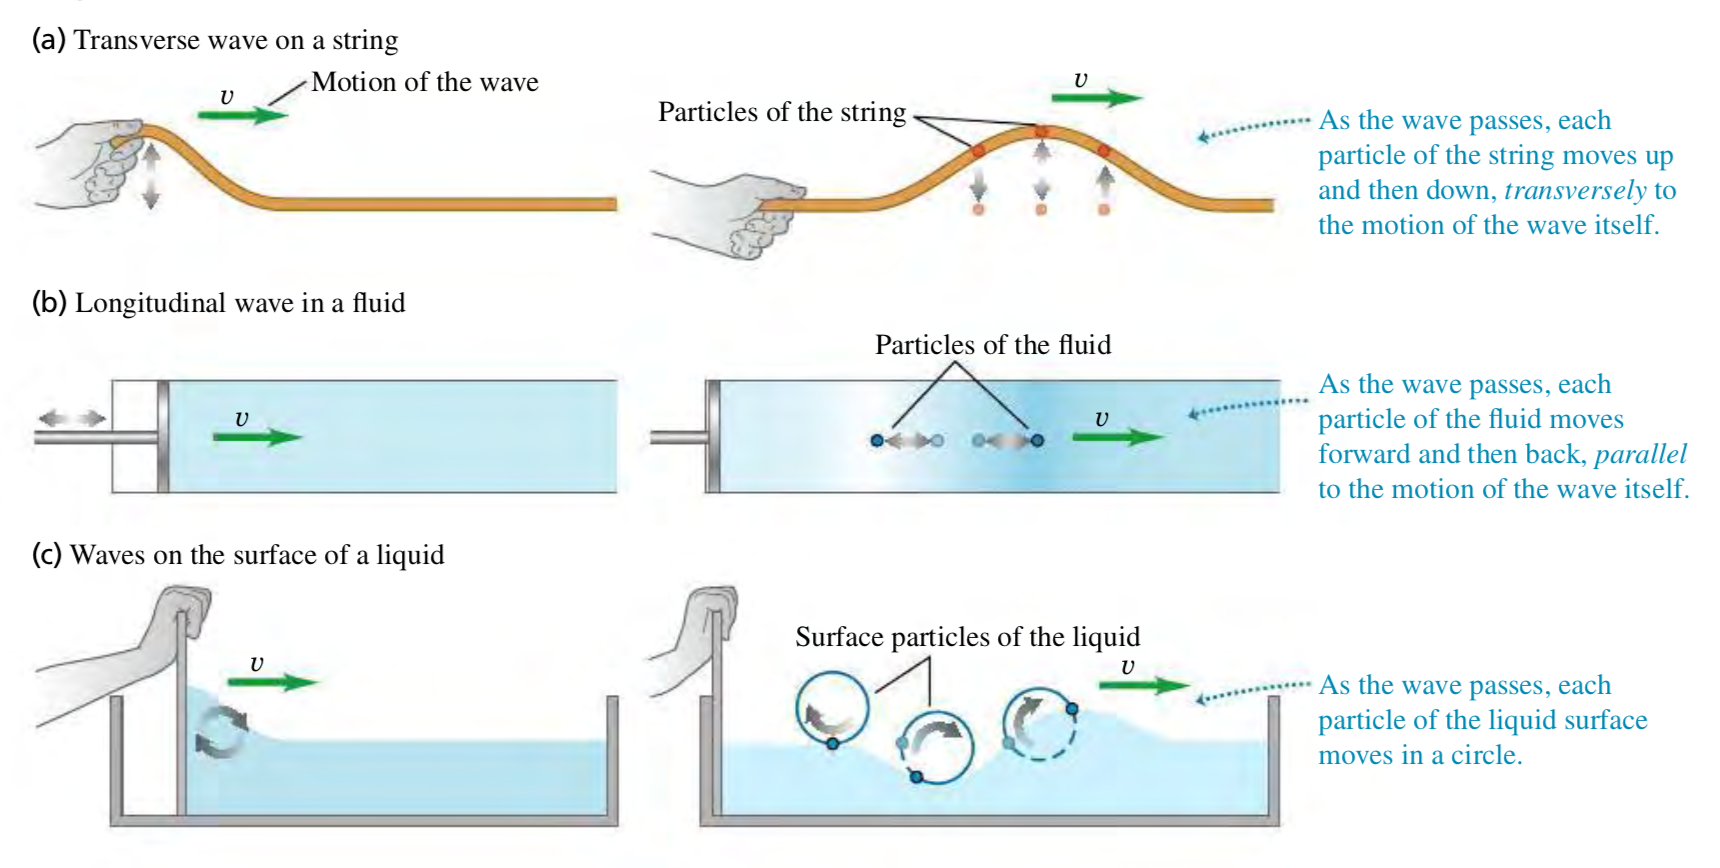
\includegraphics[scale=0.55]{images/mech_waves.png}

    \item Waves that have displacements of the medium perpendicular to to their direction
        of travel are called transverse waves while waves that have displacement in
        the direction of motion are called longitudinal waves
    \item Waves transport energy, not matter from one region to another
\end{itemize}

\section[15.2, Periodic Waves]{Periodic Waves}

\subsection{Periodic Tranverse Waves}

\begin{itemize}
    \item Suppose you move a string up and down with simple harmonic motion. The wave
        that results is a symmetric sequence of crests and troughs. These waves are
        called sinusoidal waves.
    \item for a periodic wave, the shape of the string at any instant is a repeating patterm,
        where the length of that pattern is $\lambda$
    \item The speed of the wave is thus given by $v = \lambda/T$
\end{itemize}

\subsection{Periodic Longitudinal Waves}
\begin{itemize}
    \item Longitudinal waves have periodic oscillation in the direction of motion, ex: pistons
        pressurizing water, where the regions of increased density are called compressions
    \item The fundamental equation $v = \lambda/T$ stil holds
\end{itemize}

\section{Mathematical Description of a Wave}
We call $y = y(x,t)$ the wave function. During wave motion a particle with equilibrium position
x is displaced some distance y in the direction perpendicular to the x-axis.

\subsection{Wave Function of Sinusoidal Wave}
\begin{itemize}
    \item Particles that lag behind one another but follow the same path are said to be phase
        shifted
    \item An example of a particle that moves from the farthest left point ($x=0$) will
        oscillate with SHM as follows: (Note that $\omega = 2\pi{}f$)
        \begin{equation}
            y(x=0,t) = A\cos\omega{}t = A\cos{}2\pi{}ft
        \end{equation}
    \item This can be generalized for a motion at $x$ at the earlier time $t - x/v$
        \begin{equation}
            y(x,t) = A\cos\bigg[\omega\bigg(t-\frac{x}{v}\bigg)\bigg]
        \end{equation}
    \item This function can also be written in terms of period $T = 1/f$ and wavelength
        $\lambda = v/f = 2\pi v/w$
        \begin{equation}
            y(x,t) = A\cos\bigg[ 2\pi\bigg(\frac{x}{\lambda}-\frac{t}{T}\bigg)\bigg]
        \end{equation}
    \item Note that $\omega = vk$
    \item It is often convenient to quantify the wave number $k = \frac{2\pi}{\lambda}$,
        then the wave equation can be rewritten as:
        \begin{equation}
            y(x,t) = A\cos(kx - \omega{}t)
        \end{equation}
    \item Note that if the wave is going in the opposite direction $(-x)$ then the whole
        equation becomes:
        \begin{equation}
            y(x,t) = A\cos\bigg[\omega\bigg(t+\frac{x}{v}\bigg)\bigg] =
            A\cos\bigg[ 2\pi\bigg(\frac{x}{\lambda}+\frac{t}{T}\bigg)\bigg]
            = A\cos(kx + \omega{}t)
        \end{equation}
    \item The quantity $(kx \pm \omega t)$ is called the phase. Wave speed is the speed
        with which a particle must move along the wave to keep alongside a point of a given phase.
        taking the derivative with respect to $t$ yields
        \begin{equation}
            \frac{dx}{dt} = \frac{\omega}{k}
        \end{equation}
\end{itemize}

\subsection{Particle Velocity and Acceleration in a Sinusoidal Wave}
\begin{itemize}
    \item The wave function can be used to get an expression for the transpose velocity of any
        particle in the transverse wave
    \item Given the wave function $y(x,t) = A\cos(kx - \omega t)$ then the derivative $v_{y}(x,t)$ is
        \begin{equation}
            v_{y}(x,y) = \frac{\partial y(x,t)}{\partial t} = \omega A\sin(kx - \omega t)
        \end{equation}
    \item The acceleration of any particle is the second partial derivative of y(x,y) with respect to t:
        \begin{equation}
            a_y(x,y) = \frac{\partial^{2}y(x,y)}{\partial t^2} = -\omega^{2}A\cos(kx-\omega t)
            = -\omega^{2}y(x,t)
        \end{equation}
    \item The second partial derivative with respect to x tells us the curvature of the string
        \begin{equation}
            \frac{\partial^{2}y(x,t)}{\partial x^{2}} = -k^2A\cos(kx - \omega t) = -k^2y(x,t)
        \end{equation}
    \item Given the relationship that $\omega = vk$ we can see that
        \begin{equation}
            \frac{\partial^2y(x,t)/\partial t^2}{\partial^2y(x,t)/\partial x^2} =
            \frac{\omega^2}{k^2} = v^2
        \end{equation}
    \item then the wave equation can be written as a second order partial differential equation of the
        form:
        \begin{equation}
            \frac{\partial^2y(x,t)}{\partial x^2} =
            \frac{1}{v^2}\frac{\partial^2y(x,t)}{\partial t^2}
        \end{equation}
    \item For longitudinal waves, the wave function $y(x,t)$ still measures displacement of a particle
        of the medium from equilibrium. But the displacement this time is parallel to the x-axis
\end{itemize}

\section[15.4, Speed of a Tranverse Wave]{Speed of a Transverse Wave}
What determines the speed of a transverse wave is the tension of the string and the mass per unit
length. Increased tension leads to an increase in restoring forces which increases speed. While
increasing the mass per unit makes the motion more sluggish and thus slowing down the speed.

\subsection{Wave Speed of a String: First Method}
\begin{itemize}
    \item Consider a flexible string, with tensions $F$ and a linear mass density of $\mu$, when
        Starting at $t=0$, if this was a point mass, then the end would move with constant acceleration.
        But here, the effect of $F_y$ is to set more and more mass in motion.

        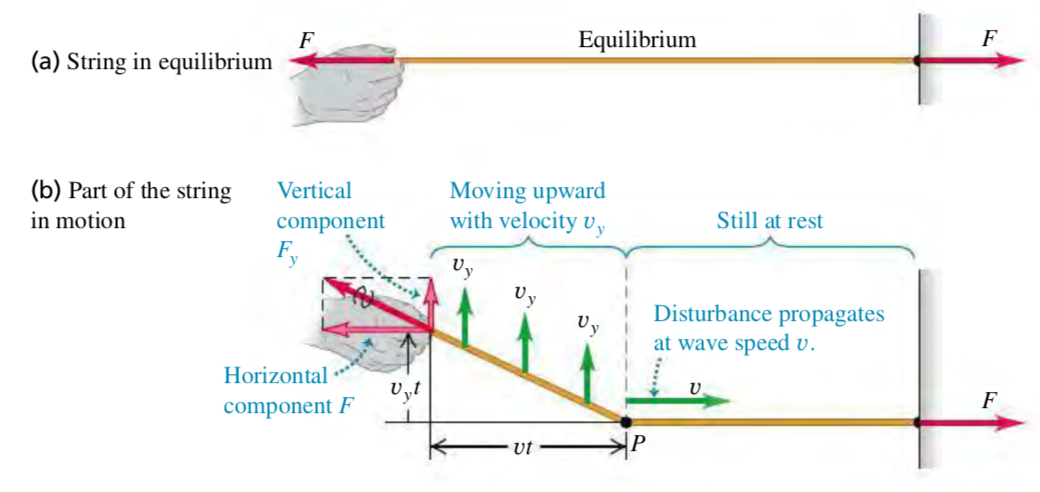
\includegraphics[scale=0.65]{images/string_transverse.png}

    \item Since the $F_{y}t$ is the impulse which is equal to the transverse momentum, we have that.
        \begin{equation}
            F_{y}t = mv_y
        \end{equation}
    \item To derive an expression for the wave speed $v$, we note that
        \begin{equation}
            \frac{F_y}{F} = \frac{v_{y}t}{vt} \Rightarrow F = F\frac{v_y}{v}
        \end{equation}
        and we have that transverse impulse equals $F_{y}t = F\frac{v_{y}}{v}t$
    \item Then the transverse momentum $= mv_y = (\mu vt)v_y = F\frac{v_{y}}{v}t$
    \item Then the wave speed v is given by
        \begin{equation}
            v = \sqrt{\frac{F}{\mu}}
        \end{equation}
        Where F is tension of the string and $\mu$ was mass per unit length
    \item Note that the second method for wave speed can be found using Newton's second law, where
        $\sum \vec{F} = m\vec{a}$
\end{itemize}

\subsection{The Speed of Mechanical Waves}
It turns out that for many types of mechanical waves, the expression of the wave speed canbe given
the same general form:
\begin{equation}
    v = \sqrt{\frac{\text{Restoring force returning the system equilibrium}}
    {\text{Inertia resisting the return to equilibrium}}}
\end{equation}

\section[15.5, Energy In Wave Motion]{Energy In Wave Motion}

\begin{itemize}
    \item Every wave motion has energy associated with it. For example, a string transfers enery
        from what part to the next during propagation.
    \item When point $a$ moves in the y-direction, the force $F_y$ does $work$ on $a$. The corresponding
        power $P$ at $a$ is thus
        \begin{equation}
            P(x,t) = F_{y}(x,t)v_{y}(x,t) = -F\frac{\partial y(x,t)}{\partial x}
            \frac{\partial y(x,t)}{\partial t}
        \end{equation}
    \item For a sinusoidal wave we have that
        \begin{equation}
            y(x,t) = A\cos(kx - \omega t)
        \end{equation}
        \begin{equation}
            \frac{\partial y(x,t)}{\partial x} = -kA\sin(kx -\omega t)
        \end{equation}
        \begin{equation}
            \frac{\partial y(x,t)}{\partial t} = \omega A\sin(kx -\omega t)
        \end{equation}
        \begin{equation}
            P(x,t) =  Fk\omega A^{2}\sin^{2}(kx -\omega t)
        \end{equation}
    \item Using the relationships $\omega = vk$ and $v^2 = F/\mu$ you can express $P(x,t)$ also as:
        \begin{equation}
            P(x,t) = \sqrt{\mu F}\omega^{2}A^{2}\sin^{2}(kx - \omega t)
        \end{equation}
    \item The maximum value of instantaneous power occurs when the $\sin^2 = 1$
        \begin{equation}
            P_{max} = \sqrt{\mu F}\omega^{2}A^{2}
        \end{equation}
    \item Note that the average power is hence given by
        \begin{equation}
            P_{av} = \frac{1}{2}\sqrt{\mu F}\omega^{2}A^{2}
        \end{equation}
\end{itemize}
\end{document}
